% Chapter Template

\chapter{Theoretical Model for QD's} % Main chapter title

\label{sec:Model} % Change X to a consecutive number; for referencing this chapter elsewhere, use \ref{ChapterX}

%----------------------------------------------------------------------------------------
%	SECTION 1
%----------------------------------------------------------------------------------------

The hole manifold is composed of two heavy holes (HH) and two light holes (LH), with $J_Z=\pm3/2$ and $J_Z=\pm1/2$ respectively. The kinetic term for both particles in bulk can be described with the Luttinger-Kohn Hamiltonian \cite{Bulaev2005,Luttinger1956} as
\begin{equation}
	\hat{T}_{\text{HH}(LH)}=\frac{\gamma_1\pm \gamma_2}{2m_0}(p_x^2+p_y^2)+\frac{\gamma_1\mp 2\gamma_2}{2m_0}p_z^2+U(x,y)+V_H(z)\; ,
\end{equation}
where $p_i$ are the usual momentum operators, $m_0$ the free electron mass, $U(x,y)$ the lateral confinement produced by the gates and $V_H(z)$ the vertical confinement produced by the interphase in the heterostructure. The effective mass depends on the Luttinger parameters, corresponding to $\gamma_1=6.95$  and $\gamma_2=2.25$ in GaAs \cite{Bogan2018}, obtaining the masses $m_{\text{HH}}(z)=0.41m_0$ and $m_{\text{LH}}(z)=0.09m_0$. If the vertical confinement, parallel to the [001] growth direction, is strong enough the hole subband split, with the HH subband lying lower in energies than the LH subband, and the mixing between them are much smaller than the other parameters of the system. This allows us to work with the perturbative Hamiltonian for a single confined HH as
\begin{equation}
	\hat{\mathcal{H}}_0=\frac{1}{2m}(p_x^2+p_y^2)+U(x,y)\; .
\end{equation}
with $m$ the effective HH mass. We must also take into account the spin-orbit coupling (SOC) given by the Hamiltonian
\begin{equation}
	\hat{\mathcal{H}}_{SO}=-\beta (\sigma_+p_-p_+p_-+\sigma_-p_+p_-p_+) + iE_\perp\alpha(\sigma_+p_-^3-\sigma_-p_+^3)\; .
	\label{eq:SOC_Hamiltonain}
\end{equation}
here we have defined the operators $p_\pm=p_x\pm ip_y$ and the combination of Pauli matrices $\sigma_{\pm}=(\sigma_x\pm i\sigma_y)/2$. The parameter $E_\perp$ denotes the effective electric field produced by the accumulation gate, and the momentum operator $\vec{p}=-i\hbar\vec{\nabla}+\frac{e^*}{c}\vec{A}$ contains the magnetic-field potential dependence with $e^*$ being the effective hole electric charge and $c$ the speed of light. The SOC consists in two different contributions: the Dresselhaus term ($\beta$) due to the bulk inversion asymmetry \cite{Dresselhaus1955} and the Rashba spin-orbit ($\alpha$) due to the structure inversion asymmetry \cite{Bychkov1984}. The coupling between HH and LH also produce a new SOC term\cite{Bulaev2007}, but it's value is much smaller that the two here commented, so we will not include it in our model. We are interested in a phenomenological model, so we can rewrite the above Hamiltonians using a simple Hubbard-Anderson \cite{1963a,Anderson1961,Traa1994} model consisting of $N$ impurities. The total Hamiltonian can be summarized as
\begin{equation}
	\hat{\mathcal{H}}=\hat{\mathcal{H}}_{\text{QD}}+\hat{\mathcal{H}}_B+\hat{\mathcal{H}}_{\text{SO}}\; ,
	\label{eq:total_Hamiltonian}
\end{equation}
with the first term representing the array of quantum dots
\begin{equation}
	\hat{\mathcal{H}}_{\text{QD}}=\sum_{i=1}^N\varepsilon_{i}\hat{c}^\dagger_i\hat{c}_i+\sum_{i=1}^NU_i\hat{n}_{i\uparrow}\hat{n}_{i\downarrow}+\sum_{i\neq j}\frac{U_{ij}'}{2}\hat{n}_i\hat{n}_j-\sum_{i\neq j,\sigma}t_{N,ij}(\hat{c}^\dagger_{i\sigma}\hat{c}_{j\sigma}+ \text{H.c.})\; .
\end{equation}
The first term on the right hand side ot the above equation represents the on-site energy $\varepsilon_{i}$ of the dot $i$, the second and third terms are the intradot $U_i$ and interdot $U_{ij}'$ Coulomb interactions respectively, which can depend on the sites. Finally the fourth term corresponds to the spin-conserving tunneling rate $t_{N,ij}$ between dots $i$ and $j$. The annihilation (creation) fermionic operators on the site $i$ and with spin $\sigma=\uparrow,\downarrow$ are given by $\hat{c}^{i\sigma}$ ($\hat{c}_{i\sigma}^\dagger$), and $\hat{n}_{i\sigma}$ is the particle number operator. To keep the computations as simpler as possible it is common to neglect the interdot Coulomb interactions, so we set $U_{ij}'=0$. In the above Hamiltonian we have only considered the ground state of each orbital, neglecting excited states. This is justified if the relevant energies are $\ll U_i$, what we will see in next section that is our case. In this work we will treat with linear arrays of QD in the approximation of first neighbour coupling, so tunneling will be only available for adjacent dots. The second term of Eq.~(\ref{eq:total_Hamiltonian}) represents the Zeeman splitting due to a magnetic filed perpendicular to the QD's plane
\begin{equation}
	\hat{\mathcal{H}}_{\text{B}}=\frac{1}{2}g^*\mu_B B_\perp\sum_{i=1}^N(\hat{n}_{i\uparrow}-\hat{n}_{i\downarrow})\; ,
\end{equation}
where $g^*$ is the effective Landé factor, $\mu_B$ is the Bohr magneton and $B_\perp$ the applied perpendicular magnetic field. It has being measured that the effective $g^*$ in QD with a hole presents an anisotropic behaviour \cite{Wang2016} with respect to the angle of magnetic field, reaching a vanishing value when the magnetic field is parallel to the QD plane. We want to keep the model simple so we will consider only a perpendicular magnetic field $\vec{B}=[0,0,B]$, so the magnetic potential $\vec{B}=\vec{\nabla}\times\vec{A}$ is set to $\vec{A}=\frac{B}{2}[-y,x,0]$. At very high magnetic field a cubic term appears in the Zeeman splitting \cite{Hung2017}, but we will not work with such a high values so we can neglect this contribution. In order to give a phenomenological expression for the SOC we use the Loewdin procedure. Imagine a double quantum dot (DQD), populated with one particle in each site, given by $\ket{L}$ and $\ket{R}$. Let us define the spatial wave function for these particles as a Gaussian shape centered in each dot separated by a distance $2d$ in the $x$ axis, and with a characteristic length $l$, so the wave functions are written as
\begin{equation}
	\begin{split}
	\ket{L}&=\frac{\sqrt{2}}{l\sqrt{\pi}}\exp(-\frac{(x-d)^2+y^2}{l^2})\; ,\\
	\ket{R}&=\frac{\sqrt{2}}{l\sqrt{\pi}}\exp(-\frac{(x+d)^2+y^2}{l^2})\; .\\
	\end{split}
\end{equation}
The characteristic length can be defined as
\begin{equation}
	\frac{1}{l^2}=\frac{m}{\hbar}\sqrt{\omega_0^2+\omega_c^2/4}\; ,
\end{equation}
where $\omega_0$ is the characteristic frequency of the harmonic confinement and $\omega_0\equiv \frac{eB}{mc}$ the cyclotron frequency due to the magnetic field applied. The overlap between the orbitals is given by
\begin{equation}
	S\equiv \braket{R}{L}=\exp(-2\frac{d^2}{l^2})\; ,
\end{equation}
what allow us to build a new basis
\begin{equation}
	\begin{split}
	\ket{\overline{L}}\equiv \ket{L}-\frac{1}{2}S\ket{R}\; ,\\
	\ket{\overline{R}}\equiv \ket{R}-\frac{1}{2}S\ket{L}\; ,\\
	\end{split}
\end{equation}
whose elements are orthogonal up to second order in the overlapping $\braket{\overline{R}}{\overline{L}}=\order{S^3}$. Looking at Eq.~(\ref{eq:SOC_Hamiltonain}) we observe that both SOC couple the spin with the orbital degree of freedom, so the tunneling of the particle must be accompanied by a flip in the spin. Now we define the states $\ket{i\uparrow}$ and $\ket{i\downarrow}$ in which the particle is located in the dot $i=L,R$ with spin up and down respectively. Computing the matrix elements $\bra{\overline{L}\uparrow}p_-p_+p_-\ket{\overline{R}\downarrow}$ and $\bra{\overline{L}\uparrow}p_-^3\ket{\overline{R}\downarrow}$ we obtain the result
\begin{equation}
	\bra{\overline{L}\uparrow}\hat{\mathcal{H}}_{\text{SO}}\ket{\overline{R}\downarrow}=-8i\beta\hbar^3\left(\frac{d}{l^4}-\frac{d^3}{l^6}+\frac{d}{16l_B^2}\right)\exp(-2\frac{d^2}{l^2})-8\hbar^3\alpha E_\perp \frac{d^3}{l^6}\exp(-2\frac{d^2}{l^2})\; ,
\end{equation}
where we have neglected terms of order higher than $\order{S^3}$ and defined the length $l_B\equiv \sqrt{\hbar/m\omega_c}$. The result corresponds to a complex number whose phase is given by the relative strength of the Rashba and Dresselhaus SOC, so we can write the spin-flip tunneling element as
\begin{equation}
	\bra{\overline{L}\uparrow}\hat{\mathcal{H}}_{\text{SO}}\ket{\overline{R}\downarrow}=t_Fe^{i\theta}\; .
\end{equation}
It can be verify that the SOC does not couple two states with the particle in the same site, i.e. $\bra{L (R)}\hat{\mathcal{H}}_{\text{SO}}\ket{L (R)}=0$. With what we have obtained we can write the third term of Eq.~(\ref{eq:total_Hamiltonian}) in the second quantization formalism as
\begin{equation}
	\hat{\mathcal{H}}_{\text{SO}}=\sum_{i\neq j\atop \sigma\neq\sigma'}(t_{F,ij}e^{i\theta_{ij}}\hat{c}^\dagger_{i\sigma}\hat{c}_{j\sigma'}+\text{H.c.} )\; .
\end{equation}
In this work we will only study a close system, i.e. without coupling the QD's to a source and a drain contacts. One of the systems that we will study in this work is a linear TQD array, in Fig.~\ref{fig:TQD_Sketch} we have plotted the possible tunneling paths for a hole confined in the system. Here we can see that the coupling between second neighbours are forbidden in our model.
\begin{figure}[!htbp]
	\centering
	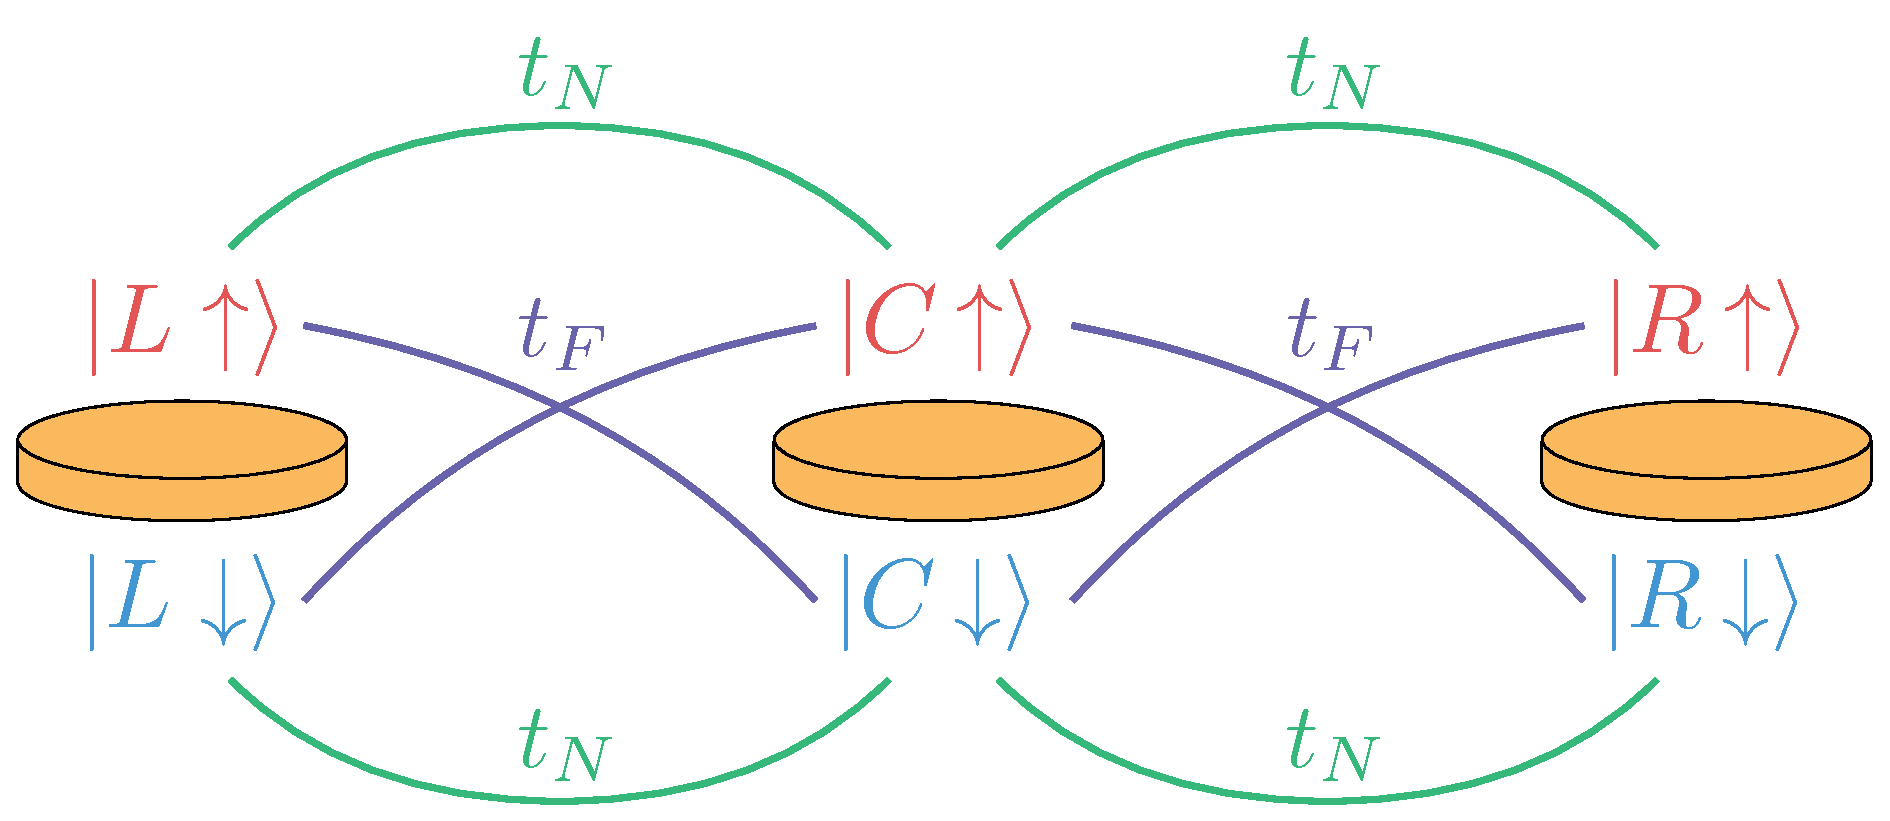
\includegraphics[width=0.5\linewidth]{TQD_Sketch.eps}
	\caption{Pictorial representation for the possible tunneling that a HH can experiment in a linear triple quantum dot array. The spin-conserving and spin-flip tunneling rates are denoted with $t_N$ and $t_F$ respectively. In principle the rates for each dot can be tuned independently.}
	\label{fig:TQD_Sketch}
\end{figure}

Due to the typical energies and times for holes in quantum dots, the units that we will use during this work are $\mu$eV for energy and ns for time. In this units the reduced Plank constant has a value of $\hbar=0.6582 \; \mu$eV$\cdot$ns.


